\section*{Dati e risultati}

\subsection*{Filtro Passa-Basso}

Per ottenere un filtro Passa-basso, illustrato in figura XXX, abbiamo montato un circuito $R\,C$ con una resistenza in serie ad un condensatore.
La caratteristica di tale filtro è quella di permettere il passaggio di tutte le frequenze che spaziano tra i $0\,\si{\hertz}$ fino alla frequenza di taglio ($\nu\ped{0}$), caratteristica propria del circuito determinata dai componenti dello stesso.
In questa prima parte ci interessa verificare pertanto che tale circuito si comporti effettivamente come un filtro passa-basso.

Noi sappiamo che la frequenza di taglio è quella frequenza che impone ad un segnale in uscita da un circuito, rispetto a quello di entrata, uno sfasamento di $\frac{\pi}{4}$ o in altri termini un'attenuazione della sua intensità di $\frac{1}{\sqrt{2}}$.
Pertanto conoscendo la relazione che sussiste tra la frequenza di taglio ($\nu\ped{0}$), la resistenza ($R$) ed il codensatore ($C$):

\begin{equation}
	\nu\ped{0} \,=\, \frac{1}{2\,\pi\,R\,C}
	\label{eq:taglio basso}
\end{equation}
%
possiamo determinare il valore della frequenza di taglio imponendo un valore di resistenza e capacità a piacere. I valori stabiliti sono i seguenti:

\begin{equation*}
	\text{Frequenza di taglio:} \quad \nu\ped{0} \,=\,
\end{equation*}
\begin{equation*}
	\text{Resistenza:} \quad R \,=\,
\end{equation*}
\begin{equation*}
	\text{Capacità:} \quad C \,=\,
\end{equation*}

Quindi una volta realizzato il circuito e note le sue caratteristiche abbiamo raccolto una serie di valori relativi alla tensione in ingresso al circuito ($V\ped{in}$), la tensione ai capi del condensatore ($V\ped{out}$) e la frequenza del segnale in uscita ($\nu\ped{out}$).
In questo modo potremo studiare la funzione di trasferimento del filtro al variare della frequanza in ingresso ($\nu\ped{in}$).

I dati ottenuti sono riportati nei seguenti grafici:

[GRAFICO]

\subsection*{Filtro Passa-Banda}

Per ottenere un filtro Passa-banda, illustrato in figura XXX, abbiamo montato un circuito $R\,C\,L$ con una resistenza in serie al parallelo tra un'induttanza ed un condensatore.
La caratteristica di tale filtro è quella di permettere il passaggio di frequenze che appartengono solo ad un determinato intervalo centrato intorno alla frequenza di risonanza ($\nu\ped{r}$), mentre atenua tutte quelle non appartenenti ad esso.
In questo caso a noi interessa ricavare, stabilita una certa frequenza di risonanza, l'intervallo di frequenze che vengono trasmesse e verificare pertato che tale circuito sia una buona approssimazione di un filtro passa-banda.

Poiche conosciamo la relazione che lega la frequenza di risonanza ($\nu\ped{r}$) con l'induttanza ($L$) e la capacità ($C$):

\begin{equation}
	\nu\ped{r} \,=\, \frac{1}{2\,\pi\,\sqrt{L\,C}}
	\label{eq:risonanza banda}
\end{equation}
%
possiamo determinare il valore della frequnza di risonanza scegliendo a piacere i valori di induttanza e capacità. Pertanto la nostra scelta è stata la seguente:

\begin{equation*}
	\text{Frequenza di risonanza:} \quad \nu\ped{r} \,=\,
\end{equation*}
\begin{equation*}
	\text{Induttanza:} \quad L \,=\,
\end{equation*}
\begin{equation*}
	\text{Capacità:} \quad C \,=\,
\end{equation*}

Quindi anche in questo caso raccoglindo, mediante l'oscilloscopio, una serie di valori relativi alla tensione in ingresso al circuito ($V\ped{in}$), la tensione ai capi del condensatore ($V\ped{out}$) e la frequenza del segnale in uscita ($\nu\ped{out}$), possiamo studiare la funzione di trasferimento del seganle al variare della frequanza in ingresso ($\nu\ped{in}$) al circuito.

I risultati da noi ottenuti sono riportati nei grafici seguenti:

\begin{figure}
  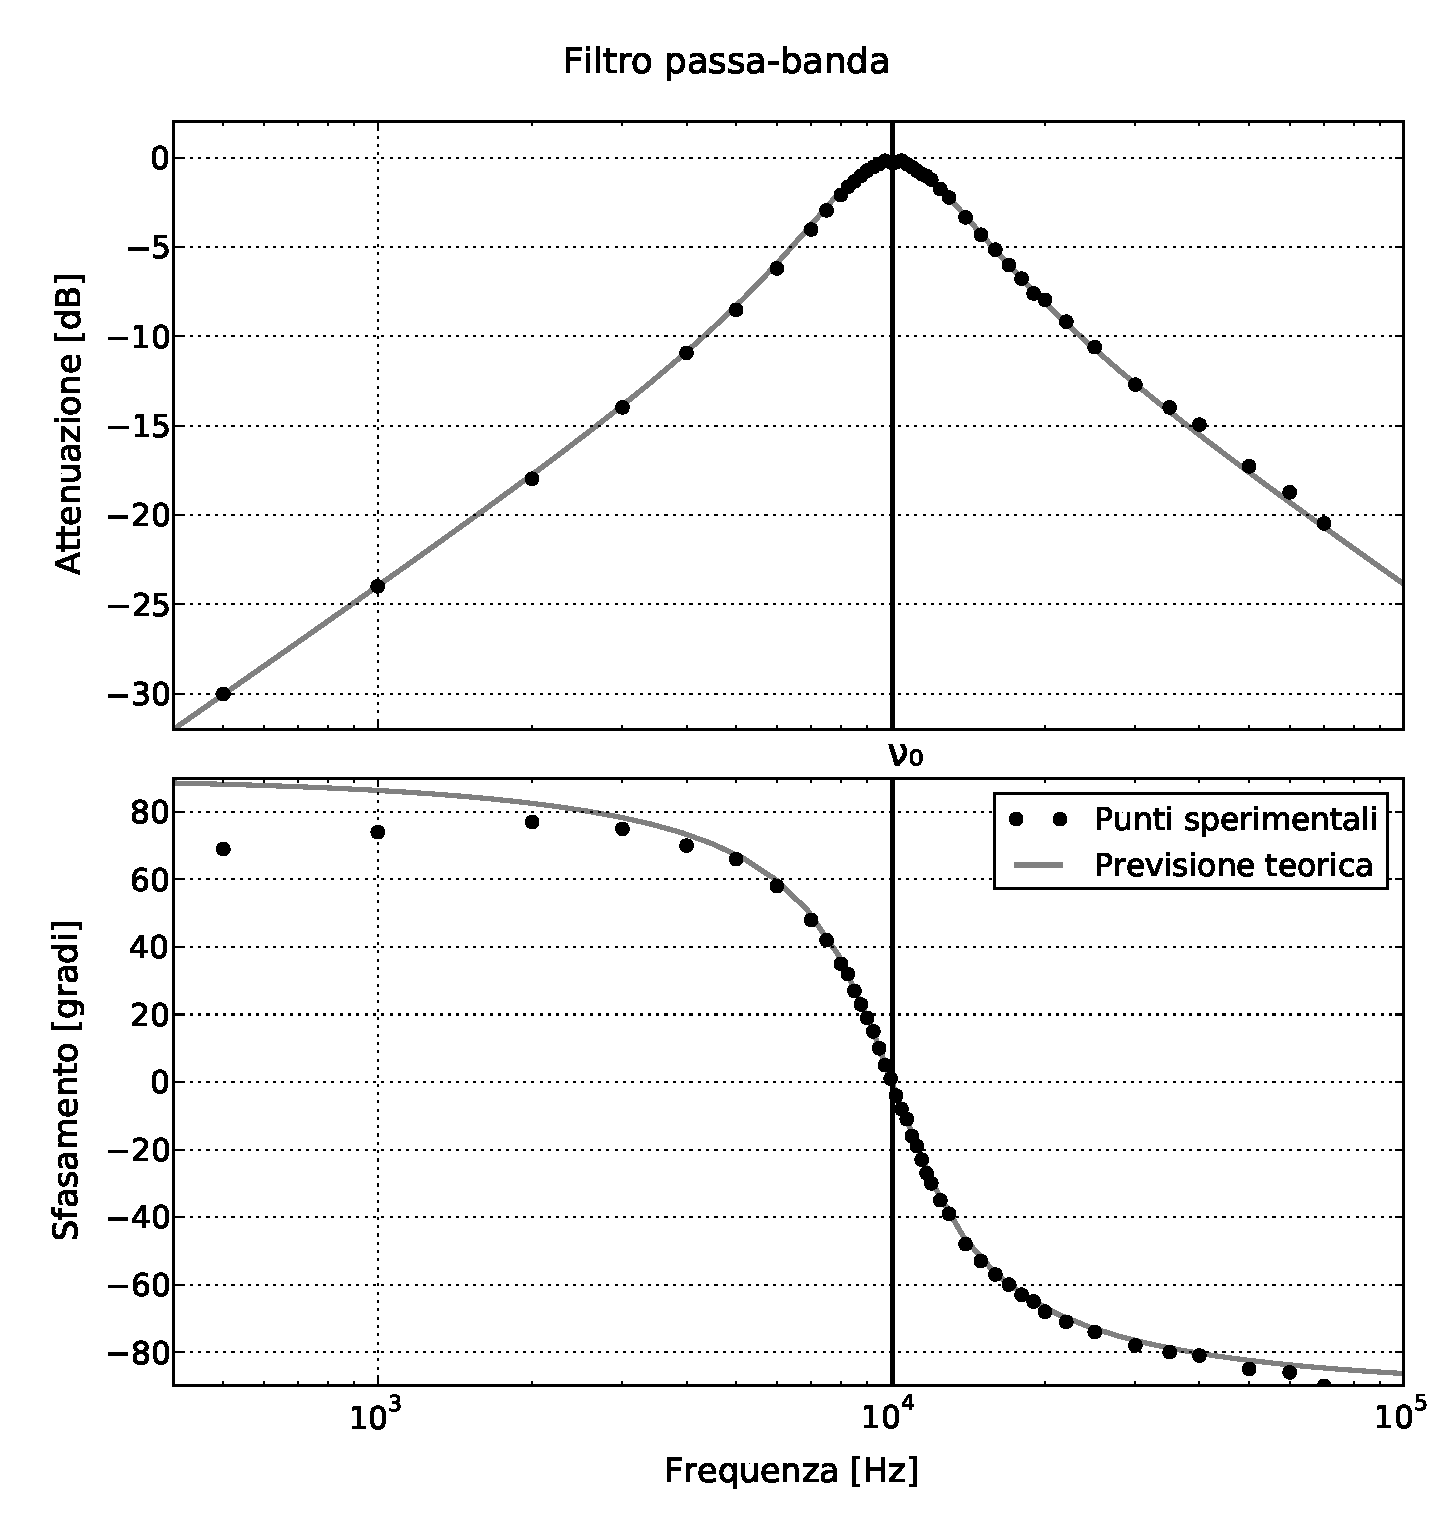
\includegraphics[scale=0.5]{passa_banda.pdf}
\end{figure}

\subsection*{Filtro a Reiezione di Banda}

Per ottenere un filtro a Reiezione di banda, illustrato in figura XXX, abbiamo montato un circuito $R\,C\,L$ con una resistenza in serie ad un'induttanza ed un condensatore.
Questo filtro non è altro che l'opposo del filtro Passa-banda ovvero, nota la frequenza di risonanza ($\nu\ped{r}$), il filtro impedisce la trasmissione delle frequenze appartenenti all'intervallo centrato su $\nu\ped{r}$. L'analisi che viene fatta per questo circuito è del tutto analoga a quella illustrata per il filtro Passa-banda, come anche i valori di capacità, induttanza e frequenza di risonanza esposti nella sezione precedente.

Pertanto i risultati ottenuti per questo circuito $R\,C\,L$ sono riportati nei seguenti grafici:

[GRAFICO]
